% !TeX spellcheck = fr_FR
\chapter{Chapitre 4 : Mesures et Performances}

Toutes les mesures de vitesse sont faites sur l'algorithme Bcrypt avec un cost de 5.

\section{Mesures CPU}

Les performances de l'attaque Bcrypt sur \gls{cpu} ont été évaluées en utilisant un programme C multi-threadé. 
Les tests ont été effectués en augmentant progressivement le nombre de threads (1, 2, 4, etc.) pour observer l'évolution de la vitesse de calcul. 

\begin{figure}[tbph!]
	\centering
	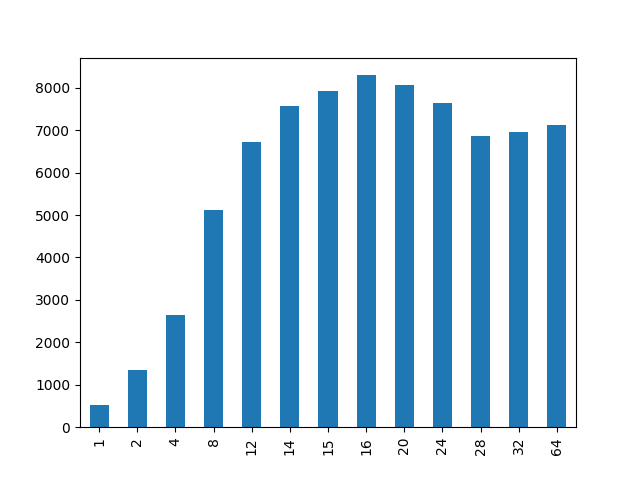
\includegraphics[width=0.7\linewidth]{stats_cpu}
	\caption[Mesures Bcrypt CPU]{Mesures Bcrypt CPU. Source : réalisé par Kandiah Abivarman}
	\label{fig:cpu_measures}
\end{figure}

Cette mesure a été faite sur un AMD Ryzen 7 4800U avec 8 Cores et 2 Threads par core.
On peut observer que le hashrate le plus élevé est à environ 8200 H/s.
Les résultats montrent une augmentation linéaire du hashrate jusqu'à un certain point, après lequel l'amélioration s'arrête en raison de la surcharge de gestion des threads.

\section{Mesures GPU}

Pour évaluer les performances de l'attaque Bcrypt sur \gls{gpu}, un benchmark a été réalisé à l'aide de Hashcat, un outil largement utilisé pour les attaques de mots de passe. 
Le test a permis de mesurer le hashrate du \gls{gpu}, qui s'est avéré être significativement supérieur à celui du \gls{cpu}, grâce à la capacité du \gls{gpu} à traiter un grand nombre de calculs en parallèle.

Les performances observées sont directement corrélées avec la puissance de calcul du \gls{gpu}, ainsi que la mémoire dédiée. 
Le tableau suivant résume les résultats obtenus avec différentes configurations de \gls{gpu}.

\begin{figure}[tbph!]
	\centering
	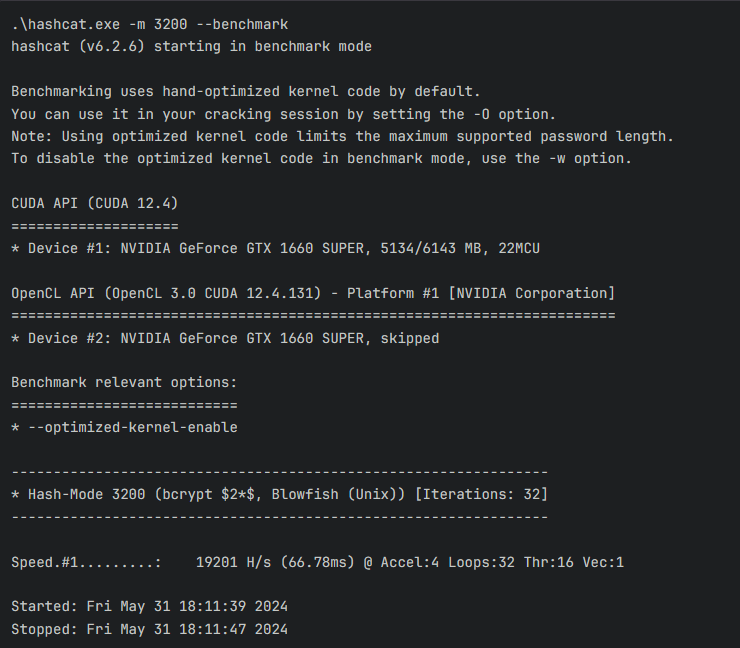
\includegraphics[width=0.7\linewidth]{gpu_benchmark}
	\caption[Mesures Bcrypt GPU]{Mesures Bcrypt GPU. Source : réalisé par Kandiah Abivarman}
	\label{fig:gpu_benchmark}
\end{figure}

La mesure a été faite sur un NVIDIA GTX 1660 Super, qui a une puissance maximale de 125 W.
Comparé au \gls{cpu}, le \gls{gpu} démontre une efficacité accrue pour cette tâche, avec un hashrate à 19201 H/s.

\section{Mesures FPGA}

Les performances de l'attaque Bcrypt sur \gls{fpga} ont été mesurées en termes de hashrate et de consommation électrique. 
D'après mes mesures, un bcrypt core prend 649'225 coups d'horloge pour un hash.

\subsection{Solution UART}

J'arrive à instancier jusqu'à 22 quadcores sur cette carte \gls{fpga}.
Toutefois, la fréquence maximale que j'arrive à mettre est de 100 MHz.
De ce fait, pour 22 quadcores, c'est-à-dire 88 Bcrypt cores, on a un hashrate de 13'554 Hash/s.

Toutefois, on pourrait encore ajouter des quadcores, mais nous somme pas limitées par les ressources mais par les contraintes de timings.

\begin{figure}[tbph!]
	\centering
	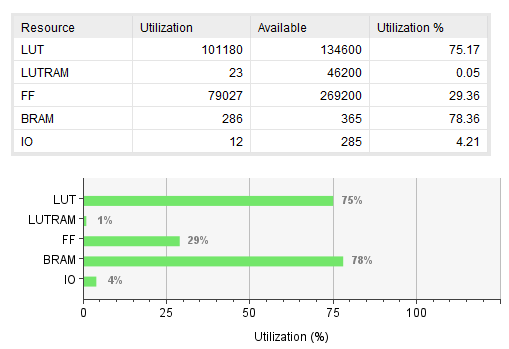
\includegraphics[width=0.7\linewidth]{nexys_ressources_22q}
	\caption[Ressources utilisés Nexys Video]{Ressources utilisés Nexys Video. Source : réalisé par Kandiah Abivarman}
	\label{fig:nexys_ressources_22q}
\end{figure}

En termes de puissance dissipés, on retrouve des résultats plutôt bon.

\begin{figure}[tbph!]
	\centering
	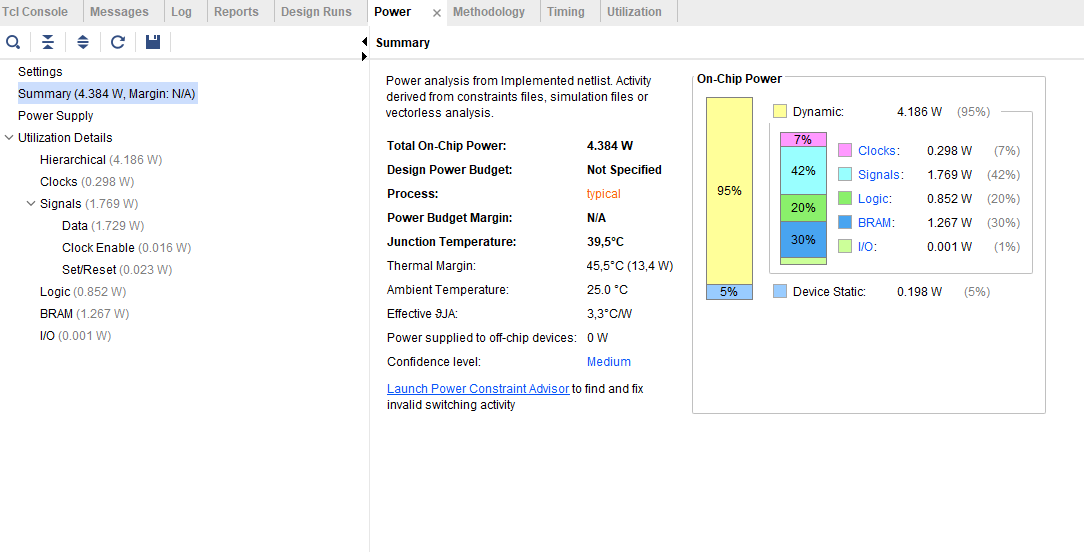
\includegraphics[width=0.7\linewidth]{nexys_22q_power}
	\caption[Mesures Puissance Max Nexys Video]{Mesures Puissance Max Nexys Video. Source : réalisé par Kandiah Abivarman}
	\label{fig:nexys_22q_power}
\end{figure}

\newpage

\subsection{Solution PCIe}

L'interface PCIe, en revanche, permet d'exploiter pleinement la puissance de l'\gls{fpga}, avec un hashrate significativement plus élevé par rapport à l'interface UART. 
En effet, contrairement à la Nexys Video, sur la KCU116, j'ai réussi à monter la fréquence d'horloge.

J'ai donc fait un tableau de mesures faites à différentes fréquences.

\begin{table}[tbph!]
    \centering
    \begin{tabular}{|l|l|l|l|l|}
    \hline
        \textbf{Freq (MHz)} & \textbf{Quadcores Max.} & \textbf{Utilisations (\%)} & \textbf{WNS} & \textbf{Hashrate (cost : 5)} \\ \hline
        100 & 36 & BRAM : 97.50, LUT : 68 & 0.988 & 22'180 H/s \\ \hline
        200 & 36 & BRAM : 97.50, LUT : 68 & 0.388 & 44'369 H/s \\ \hline
        250 & 36 & BRAM : 97.50, LUT : 68 & 0.115 & 55'450 H/s \\ \hline
        275 & < 30 & - & - & < 50'820 H/s \\ \hline
        300 & 5 & BRAM : 13.54, LUT : 7.87 & 0.007 & 9241 H/s \\ \hline
        325 & 0 & 0 & X & - \\ \hline
    \end{tabular}
	\caption{Mesures de hashrate sur KCU116}
	\label{tab:hashrate_measures}
\end{table}

On peut observer qu'à 250 MHz, on atteint un hashrate de 55'450 H/s avec 36 Quadcores.

Cependant, cette solution requiert une consommation électrique plus importante que la solution \gls{uart}. 

\begin{figure}[tbph!]
	\centering
	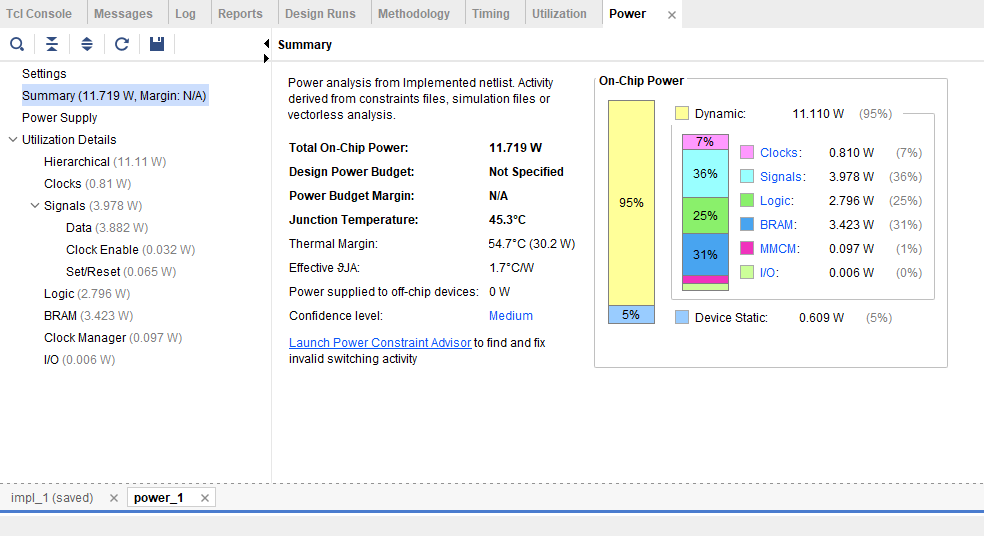
\includegraphics[width=0.7\linewidth]{kcu116_36q_power}
	\caption[Mesures Puissance Max KCU116]{Mesures Puissance Max KCU116. Source : réalisé par Kandiah Abivarman}
	\label{fig:kcu116_36q_power}
\end{figure}

En effet, on peut voir une puissance Max. de 11.7 W.


\subsection{Comparaisons}

Dans cette section, je vais comparer les performances des différentes architectures (\gls{cpu}, \gls{gpu}, \gls{fpga}) en termes de hashrate et de consommation électrique. 
Ces comparaisons permettent de mettre en évidence les points forts et les faiblesses de chaque solution pour l'attaque Bcrypt avec un cost de 5.

\subsubsection{Comparaison du Hashrate}

Le tableau présente une comparaison des hashrates obtenus pour chaque solution :

\begin{table}[tbph!]
    \centering
    \begin{tabular}{|l|l|}
    \hline
        \textbf{Architecture} & \textbf{Hashrate (H/s)} \\ \hline
        CPU (AMD Ryzen 7 4800U, 16 threads) & 8'200 H/s \\ \hline
        GPU (NVIDIA GTX 1660 Super) & 19'201 H/s \\ \hline
        FPGA (Nexys Video, 22 Quadcores, 100 MHz) & 13'554 H/s \\ \hline
        FPGA (KCU116, 36 Quadcores, 250 MHz) & 55'450 H/s \\ \hline
    \end{tabular}
    \caption{Comparaison des hashrates pour différentes architectures.}
    \label{tab:hashrate_comparison}
\end{table}

Les résultats montrent que le \gls{fpga} avec interface PCIe à 250 MHz est la solution la plus performante en termes de hashrate, atteignant 55'450 H/s, suivi par le \gls{gpu} NVIDIA GTX 1660 Super avec un hashrate de 19'201 H/s. 
Le \gls{cpu} et le \gls{fpga} avec interface UART ont des performances moindres, avec respectivement 8'200 H/s et 13'554 H/s.

\subsubsection{Comparaison de la Consommation Électrique}

Le tableau présente une comparaison des consommations électriques maximales mesurées pour chaque solution :

\begin{table}[tbph!]
    \centering
    \begin{tabular}{|l|l|}
    \hline
        \textbf{Architecture} & \textbf{Consommation (W)} \\ \hline
        CPU (AMD Ryzen 7 4800U, 16 threads) & Environ 25 W \\ \hline
        GPU (NVIDIA GTX 1660 Super) & 125 W \\ \hline
        FPGA (Nexys Video, 22 Quadcores, 100 MHz) & 4.38 W \\ \hline
        FPGA (KCU116, 36 Quadcores, 250 MHz) & 11.7 W \\ \hline
    \end{tabular}
    \caption{Comparaison des consommations électriques pour différentes architectures.}
    \label{tab:power_comparison}
\end{table}

La comparaison montre que le \gls{fpga}, particulièrement la solution Nexys Video avec interface UART, est de loin la solution la plus économe en énergie, avec une consommation de seulement 4.38 W. 
Le \gls{gpu} GTX 1660 Super, bien que performant en termes de hashrate, consomme 125 W, ce qui est significativement plus élevé. 
Le \gls{fpga} avec interface PCIe, bien qu'il consomme plus que la solution UART, reste plus économe que le \gls{gpu} avec une consommation de 11.7 W.

\subsubsection{Efficacité Énergétique}

L'efficacité énergétique, mesurée en termes de Hashes par joule (H/J), est un critère important pour évaluer la performance globale des différentes solutions. 
Le tableau résume ces données :

\begin{table}[tbph!]
    \centering
    \begin{tabular}{|l|l|}
    \hline
        \textbf{Architecture} & \textbf{Efficacité Énergétique (H/J)} \\ \hline
        CPU (AMD Ryzen 7 4800U, 16 threads) & 328 H/J \\ \hline
        GPU (NVIDIA GTX 1660 Super) & 154 H/J \\ \hline
        FPGA (Nexys Video, 22 Quadcores, 100 MHz) & 3'094 H/J \\ \hline
        FPGA (KCU116, 36 Quadcores, 250 MHz) & 4'739 H/J \\ \hline
    \end{tabular}
    \caption{Comparaison de l'efficacité énergétique (Hashes par joule).}
    \label{tab:efficiency_comparison}
\end{table}

Les résultats montrent que les solutions \gls{fpga}, particulièrement avec l'interface PCIe, offrent la meilleure efficacité énergétique, atteignant jusqu'à 4'739 H/J. 
Bien que le \gls{gpu} offre un bon hashrate, son efficacité énergétique est inférieure, à seulement 154 H/J, ce qui le rend moins intéressant pour des applications où la consommation d'énergie est critique. 
Le \gls{cpu} a une efficacité énergétique légèrement meilleure que le \gls{gpu}, mais reste loin derrière les \gls{fpga}.

\newpage

\subsubsection{Consommation Énergétique sur 24 Heures}

Le graphique ci-dessous montre l'évolution de la consommation énergétique en wattheures (Wh) pour chaque architecture sur une période de 24 heures.

\begin{figure}[tbph!]
    \centering
    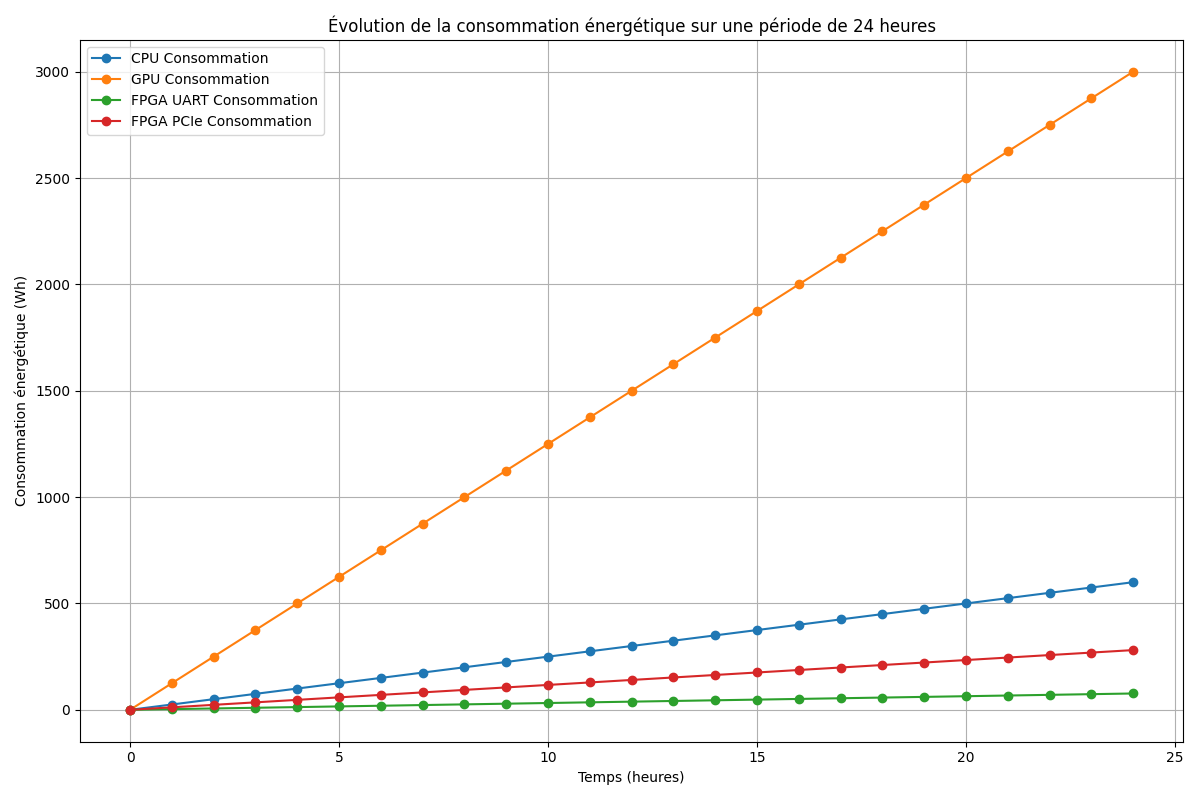
\includegraphics[width=0.7\linewidth]{power_graph_comparison.png}
    \caption[Évolution de la consommation énergétique sur 24 heures]{Évolution de la consommation énergétique en Wattheures (Wh) pour le \gls{cpu}, le \gls{gpu}, et les solutions FPGA (UART et PCIe) sur une période de 24 heures. Source : réalisé par Kandiah Abivarman}
    \label{fig:power_graph_comparison}
\end{figure}

Le graphique montre comment la consommation énergétique s'accumule au fil du temps pour chaque architecture.
On peut donc observer l'évolution dans le temps, qui est un facteur important étant donnée qu'une attaque par bruteforce peut prendre beaucoup de temps.
L'observation la plus flagrante est la différence du \gls{gpu} par rapport aux autres.

\subsubsection{Conclusion des Comparaisons}

En résumé, chaque architecture présente des avantages spécifiques. 
Le \gls{fpga} avec interface PCIe est la solution la plus performante en termes de compromis entre hashrate et efficacité énergétique. 
Le \gls{gpu}, malgré son hashrate relativement élevé, présente une efficacité énergétique inférieure aux autres. 
Le \gls{cpu}, bien qu'il soit la solution la moins performante, est toujours utile pour des applications généralistes. 
Le \gls{fpga} avec interface UART offre une solution extrêmement économe en énergie, idéale pour un environnement à faible consommation.